 
\setlength{\tabcolsep}{10pt}
\begin{table*}
\centering
\begin{tabular}{ccccc}
\hline
   Model subset & D$_{max}$ [lyr] & $\tau_a$ interval [yr] & $\tau_s$ interval 
   [yr]& description  \\
\hline
M1 & 40000 & [10000, 30000]   & [10000, 50000]   &dense, short lifetime\\
M2 & 40000 & [170000, 190000] & [10000, 50000]   &sparse, short lifetime\\
M3 & 40000 & [10000, 30000]   & [400000, 440000] &dense, long lifetime \\
M4 & 40000 & [170000, 190000] & [400000, 440000] &sparse, long lifetime\\
%
M5 & 80000 & [10000, 30000]   & [10000, 50000]   &dense, short lifetime\\
M6 & 80000 & [170000, 190000] & [10000, 50000]   &sparse, short lifetime\\
M7 & 80000 & [10000, 30000]   & [400000, 440000] &dense, long lifetime \\
M8 & 80000 & [170000, 190000] & [400000, 440000] &sparse, long lifetime\\
%
\hline
\end{tabular}
\caption{Selected models to analyze the behavior of simulation outputs
   and their dependence on simulation outputs and their dependence on
   simulation parameters.}
\label{T_selected_models}
\end{table*}

 

\begin{figure*} % 2D color plot
   \centering
   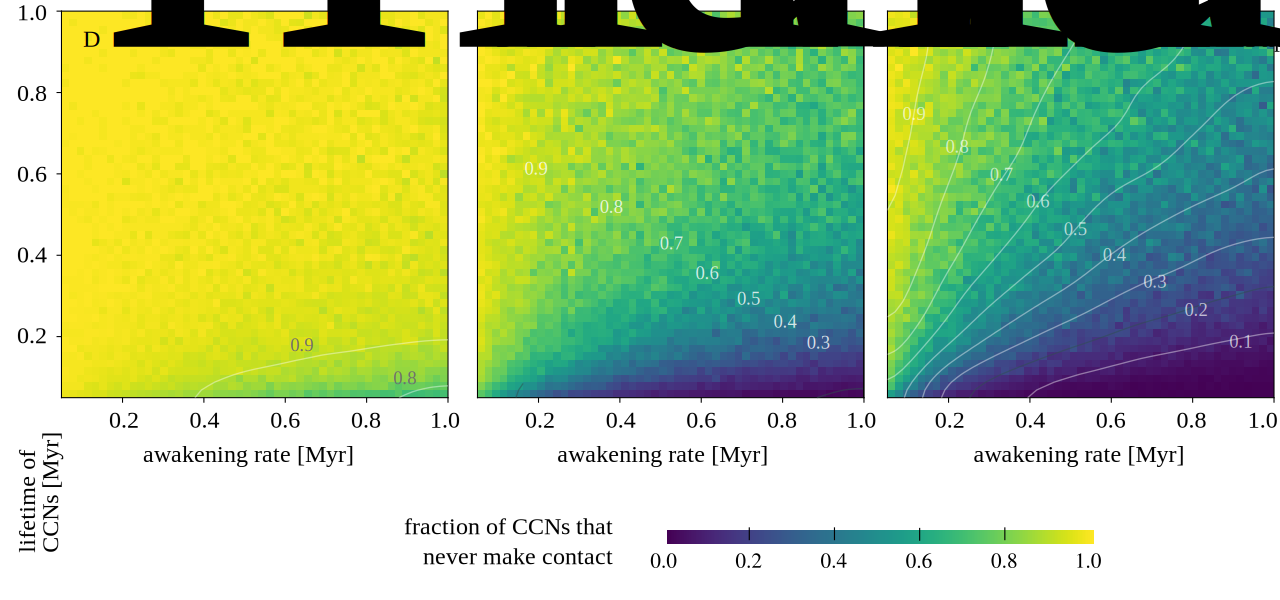
\includegraphics[width=\textwidth]{F_never_contact.pdf}
   \usecaption{F_never_contact}
   \label{F_never_contact}
\end{figure*}
 
\begin{figure*} % 2D color plot
   \centering
   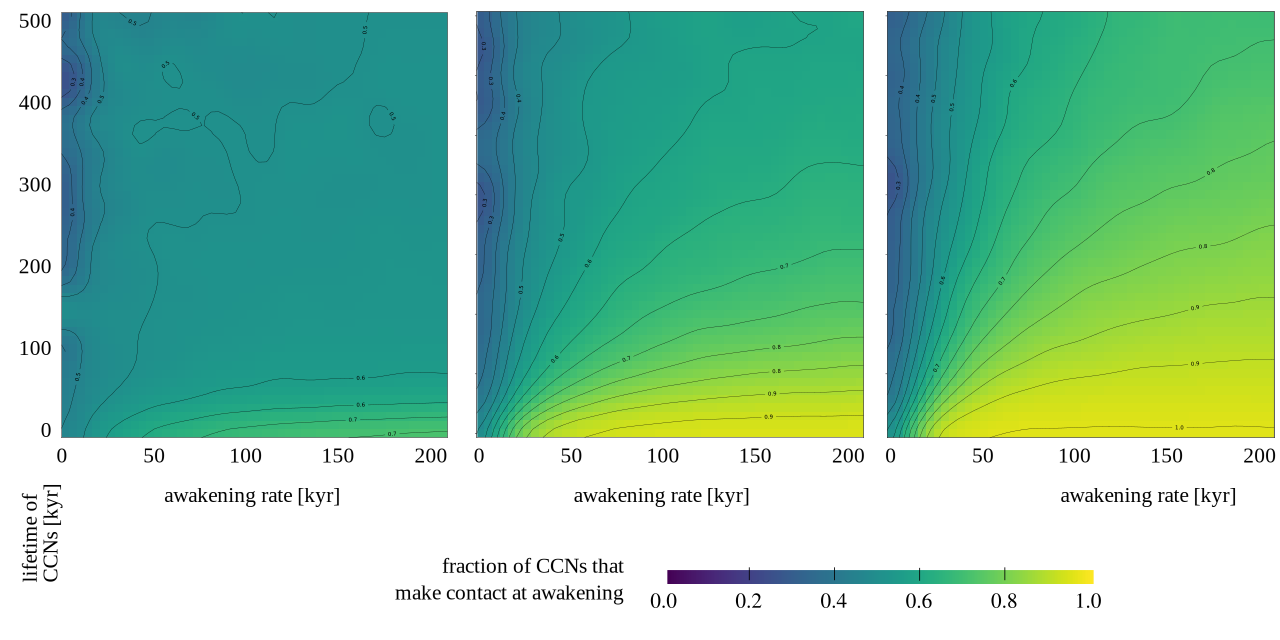
\includegraphics[width=\textwidth]{F_C_at_A.pdf}
   \usecaption{F_C_at_A}
   \label{F_C_at_A}
\end{figure*}
 
\begin{figure}
   \centering
   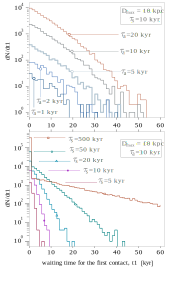
\includegraphics[width=0.5\textwidth]{F_waiting_for_1C.pdf}
   \usecaption{F_waiting_for_1C}
   \label{F_waiting_for_1C}
\end{figure}

 

%%% S E C T I O N - - - - - - - - - - - - - - - - - - - - - - -
\section{Results: exploring the parameter space}\label{S_results}
%{{{

We implemented the simulation of a regular grid of models varying over
the hypothesis space, which covers 15000 different models.
%
For each model, we simulated 50 realizations with different random
seeds, in order to perform a MonteCarlo estimation of the variance.
%
The parameters for the temporal aspects of the simulation (the mean
waiting time for the next awakening, $\left<\tau_a\right>$, and the
mean lifetime, $\left<\tau_s\right>$) cover the ranges 4000-200000 yr
and 10000-500000 yr, respectively, with a regular partition of 50
values for each parameter.
%
For the D$_{max}$ parameter, we chose the values 500, 1000, 10000,
20000, 40000 and 80000 lyr.
%
This setup makes a total of 750000 simulations, each covering a time
range of one million years.
%
\ttn{1}
%
In Table \ref{T_simu_hypotheses} we show the three variable
parameters, the ranges of their values and the number of bins that
have been explored in the numerical experiments.
%
We also show the set of parameters that take part in the simulation,
their values and the hypotheses that define the runs of the
simulations.




As a product of the simulations, several quantities can be obtained.
%
Some quantities are directly derived from the discrete events, namely,
the ID of emitting and receiving \cetis{}, the position in the galaxy, and
the times of each of the events that are relevant to keep track of the
number of \cetis{} (time of awakening and time of doomsday) and of the
number of contacts (the times of contacts and the times of blackouts).
%
We can also derive the additional quantities that represent the
properties of the \cetis{}, for example the total time elapsed between the
awakening and the doomsday of each \ceti{}.
%
The time span of a \ceti{} listening another or being listened by another
can also be easily derived from the results of a realization.
%
This way we can also compute the distribution in the galaxy of
\cetis{}
that reach contact and the waiting time until the first contact or the
waiting time until the next contact.
%
Regarding the properties of the population of \cetis{} and its evolution,
the simulation yields the fraction of awaken time a \ceti{} is listening
at least another \ceti{} (i.e., in their causal cone), the age of
contacted \cetis{} at first contact, the distribution of time to wait
until next contact, the fraction of \cetis{} where the first contact is
given at the awakening, the distribution of the number of contacts for
each \ceti{}, the distribution of the number of contacts as a function of
\ceti{} age, the number of contacts as a function of time in the galaxy,
the rate of \cetis{} that succeed in contact, and the distribution of
distances between contacted \cetis{}.
%
Another useful derived quantity is the duration of two-way
communication channels or the fraction of contacts that admit a
response.
% 
It is also possible to analyze the relations between the distance to
\ceti{} vs. the time of double communication, the distance to \ceti{} vs. the
age of contacted \ceti{}, the age of a \ceti{} and the maximum number of
contacted \cetis{} before doomsday, or the lifespan of a \ceti{} vs. the
maximum number of contacts.
%
In addition, all these quantities can be analyzed as a function of the
simulation parameters.
%
We chose eight models that are on fairly opposed regions of the
explored parameter space, and cover short/long lifetimes, short/long
waiting times for the next \ceti{} to appear in the Galaxy and short/large
range reach of the signal, including all possible combinations.
%
\ttn{2}
%
The details of each model are summarized in the
Table~\ref{T_selected_models}.


In what follows, we focus on the analysis of the duration of contacts
(Sec.~\ref{SS_multiplicity}), the waiting time for the first contact
(Sec.~\ref{SS_waiting}) and the
variations of contact possibilities as a function of the position of
the \ceti{} in the Galaxy (Sec.~\ref{SS_location}).

%}}}


\subsection{Membership to the network of connected \cetis{}}\label{SS_members}

%{{{

\ffn{3}
%
In Fig.~\ref{F_number_of_contacts} we show the empirical cumulative
distributions of the number contacts for \cetis{} in six different
samples, including short and long lifetimes
$\left(\,\left<\tau_s\right>=\right.$10000~yr and
$\left<\tau_s\right>$=100000~yr, respectively$\left.\right)$, dense
and sparse spatial distribution
$\left(\,\left<\tau_a\right>=\right.$10000~yr and
$\left<\tau_a\right>$= 100000~yr, respectively$\left.\right)$, and two
different signal reach ranges (D$_{max}$=40000 lyr and
D$_{max}$=80000~lyr).
%
The models M1 and M5 are not shown, since in both cases the total
number of contacts is different from zero for less than the five per
cent of the \cetis{}.
%
The areas between models with the same mean lifetime and mean
awakening time are shaded for visualization purposes.
%
As it can be seen from this Figure, the mean lifetime is more
determinant than the mean awakening rate (dense and sparse,
represented by a different shade) for the number of contacts.
%
As expected, of the samples with the longest $D_{max}$ the model with
a dense awakening in the timeline (low $\left<\tau_a\right>$) and a
long lifetime (high $\left<\tau_s\right>$), is the model that
maximizes the number of contacts, reaching a maximum of order 20
contacts for a single \ceti{}.
%
Similarly, for the models with long signal range
($D_{max}=80000\,lyr$), the one which is dense and with long lifetime
has the maximum number of contacts, reaching nearly 100 contacts for
each \ceti{} in its entire lifetime.
%
This is considerably larger than any model with a shorter lifetime,
which produce a number of contacts of at most the order of ten
contacts per \ceti{}.
%
A couple of comments are worth to mention about this plot, namely, it
has a logarithmic scale on the x-axis, and it is the cumulative, not
differential, empirical distribution, so that the differences in the
number of contacts for different models is quite large.
%
Another interesting feature observed in this Figure, is that for the
models analyzed, there are \cetis{} that have no causal contacts with
any other \ceti{} during their whole lifetime.
%
The fraction of \cetis{} with no contact ranges from nearly 20\% up to
nearly 90\% (models M1 and M5, not shown), except for the dense and
long lifetime models, for which almost all \cetis{} make at least one
contact.
%
Since these results depend on just eight models, we analyze the
properties of the frequency of contacts as a function of both the mean
lifetime and the mean awakening time.
%
\ffn{4}
%
On Fig.~\ref{F_never_contact} we show 2D color maps with the fraction
of \cetis{} in the simulations that never make contact (i.e., never
listen to another \ceti{}), as a function of the mean lifetime
($\left<\tau_s\right>$, in the range 0--500 yr) and the mean awakening
time ($\left<\tau_a\right>$, in the range 0--200 yr), for three
different values of the maximum signal range, $D_{max}=10000$~yr (left
panel), $D_{max}=40000$~yr (middle panel), and $D_{max}=80000$~yr
(right panel).
%
A clear pattern emerges in this Figure, showing that the probability
for a \ceti{} of making causal contact with at least another \ceti{}
during their entire lifetime, increases with increasing $D_{max}$,
increasing $\left<\tau_s\right>$ and decreasing $\left<\tau_a\right>$,
following a roughly linear dependence with the three parameters.


While the number of \cetis{} that do not succeed in reaching the
causal contact regions of other node is a useful indicator of
degree of isolation, there is also the chance that a number of
\cetis{} are already in the causal contact region of other nodes,
which shows a somewhat oposite situation.
%
\ffn{5}
%
The fraction of \cetis{} that make the first contact at the awakening
event is shown in the Fig.~\ref{F_C_at_A}, 
as a function of the mean lifetime
($\left<\tau_s\right>$, in the range 0--500 yr) and the mean awakening
time ($\left<\tau_a\right>$, in the range 0--200 yr), for three
different values of the maximum signal range, $D_{max}=10000$~yr (left
panel), $D_{max}=40000$~yr (middle panel), and $D_{max}=80000$~yr
(right panel).
%
These probabilities are consistent with the ones on the previous
Figure.
%
Although they are not complementary, it is clear that the dependence
with the three parameters is roughly linear in both cases.
%
%% DISCUTIR ESTOS RESUOLTADOS SEGUN LA LITERATURA


%

%}}}
 



\subsection{Waiting time for a first contact}\label{SS_waiting}
%{{{

In this subsection we analyze the distribution of the waiting times for
a first contact.
%
Such distribution can be considered to compute the probability for a
random \ceti{} to carry out a SETI project and spend a given time until
the first contact is made. 

\ffn{6}
%
In the Fig.~\ref{F_waiting_for_1C} we show the histograms of the mean
waiting times for the first contact, for several models.
%
Upper panel (a) panel shows the histograms for several values of the
mean survival time $\tau_s$, and the mean awakening time $\tau_a$ in
the range 68000-100000 yr.
%
Lower panel (b) shows the histograms for several values of $\tau_a$,
and $\tau_s$ in the range 17000-24000 yr.
%
As it can be seen, the shape of the histograms is almost the same when
$\tau_a$ is modified (panel (b)), but significantly changes when
$\tau_s$ is modified (panel (a)). 
%
For different values of $\tau_a$, the shape of the distribution is
similar, and the main difference is given by the different number of
contacts on the different models.
%
Conversely, for different values of $\tau_a$, the shape of the
distribution is similar, and the main difference given by the
different number of contacts on the different models. 
 

The fraction of the \cetis{} that have made at least one contact as a
function of the elapsed time since the awakening, is computed with
respect to the total number of nodes that make causal contact at least
one time in the time range from the Awakening up to the Doomsday
events.
%
From a frequentist approach, the total counts from the awakening
($t=$0~yr) up to a given time are related to the estimation of the
probability of listening during that time interval and reaching to
causal contact region of at least another node.
%
The complement of this value is the probability of observing in a time
interval with no success, i.e., without ever happening a Contact
event.
%
Clearly, this probability diminishes with time and tends to zero for
large time periods.
%             
The diferential probability of making a causal contact reach its
maximum at the awakening event for all models.
%
That is, for a short period of time like the nearly 50 years SETI
programs have been active, the initial moment is the most promising
for making a (causal) contact, at least for a given technology.
%
This consideration offers a new approach for SETI programs, where the
search for new communication technologies has a fundamental role.
%
Moreover, as it can be seen in the Fig.~\ref{F_waiting_for_1C}, there
is a maximum probability of making the first causal contact at nearly
100000 years.
%
Remarkably, the probability of such a contact does not grows linearly
with the observing time, but is greater during the first 100
millennia.



%}}}

%\subsection{Location within the Galaxy}\label{SS_location}
%%{{{
%    
%%On the Figure~\ref{F_radial_frac} we show the fraction of \cetis{} that
%%make zero, one, two or three contacts, as a function of the
%%galactocentric distance, for model M1.  VERIFICAR!  M1?
%%
%For this model, the majority of \cetis{} do not make any contact during
%all the time period in which they are active.
%%
%As expected, the fractions of \cetis{} making at least one contact
%diminishes as the number of contacts rises.
%%
%The shape of this distribution is a result of the geometry of the GHZ.
%%
%In general, a closer position to the center of the Galaxy slightly
%favours the possibility of a contact.
%%
%This would indicate that the position of the Earth is suitable for the
%odds of making a contact.
%
%%}}}
%
%

